\subsection{Bridge (\textit{o Handle, Body})}
\label{bridge}

\textbf{Scopo}: Strutturale \\
\textbf{Raggio d'azione}: Oggetti

\paragraph{Definizione} Disaccoppia un’astrazione dalla sua implementazione in modo che le due possano variare indipendentemente l’una dall’altra. È spesso utilizzato all’inizio di un progetto per consentire ad astrazioni ed implementazioni di variare in modo indipendente.

\paragraph{Problema} Quando un’astrazione può avere una tra più implementazioni possibili, in genere si risolve il problema ricorrendo all’ereditarietà. L’astrazione viene definita da un’interfaccia o da una classe astratta e le sottoclassi concrete la implementano in modi differenti. Tale approccio non è flessibile poichè l’ereditarietà lega un’implementazione ad un’astrazione in modo permanente. Ciò rende difficile modificare, estendere e riusare astrazioni ed implementazioni in modo indipendente.

\paragraph{Esempio} Si supponga di volere scrivere un toolkit per la realizzazione di interfacce grafiche. Sicuramente ci sarebbe il bisogno di un’astrazione Window per rappresentare una finestra. Si vuole far in modo che il toolkit funzioni con diversi gestori grafici come ad esempio X Windows o IBM Presentation Manager.

\begin{figure}[H]
    \centering
    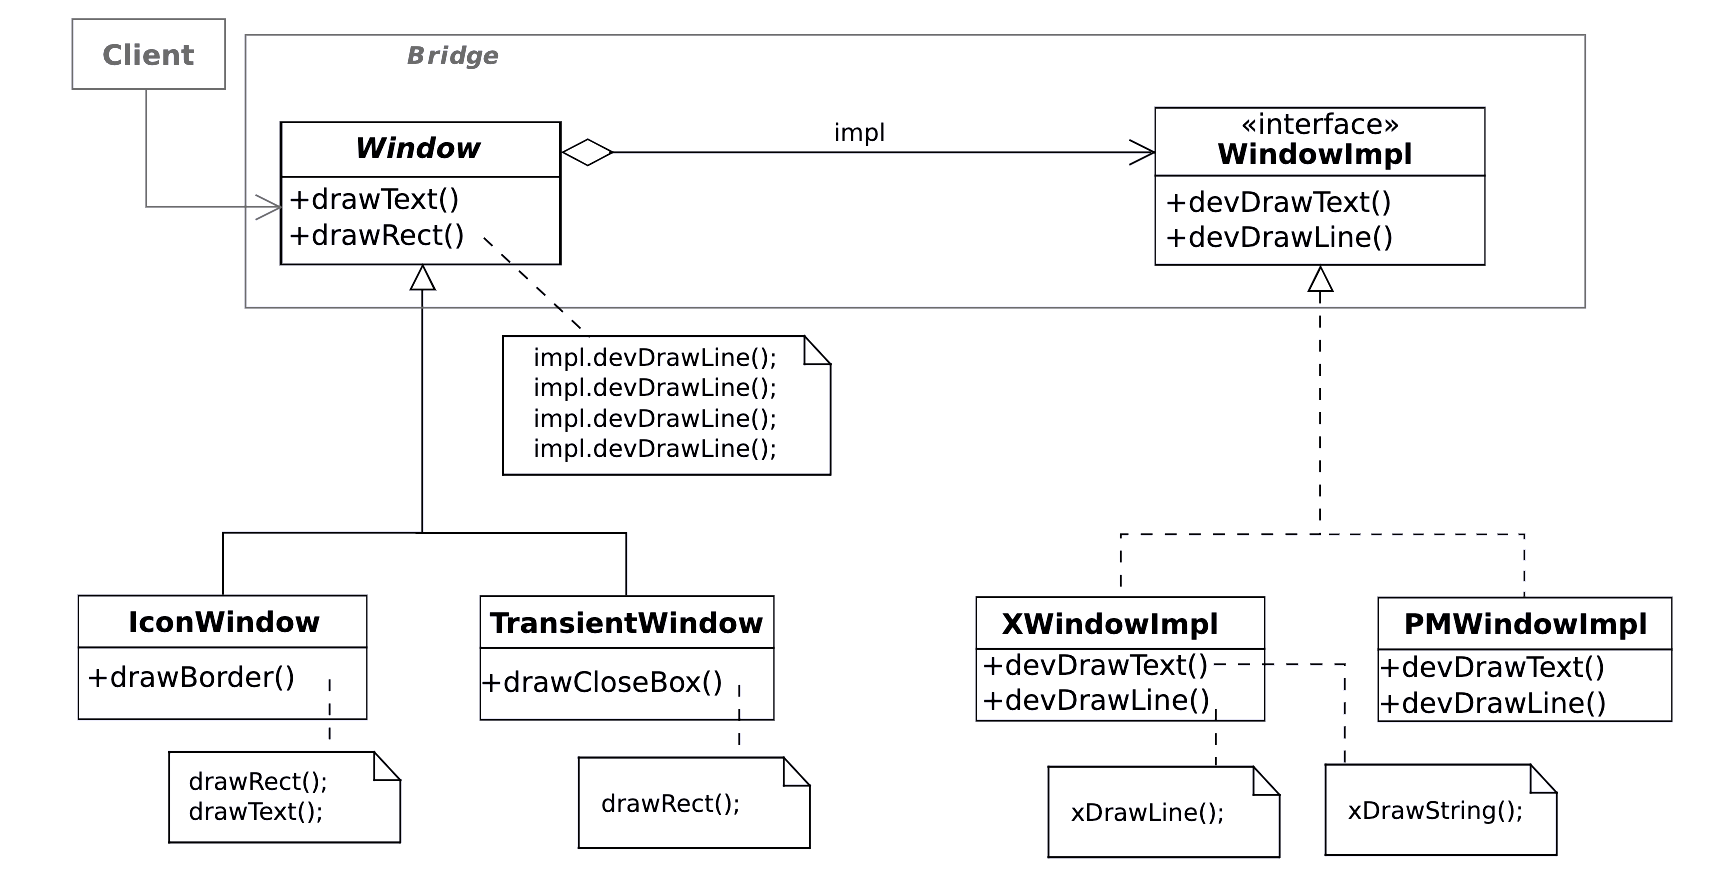
\includegraphics[width=1\linewidth]{assets/pattern/bridge/bridge-esempio.png}
\end{figure}

Si può fare ricorso all’ereditarietà rendendo Window una classe astratta (o un’interfaccia) ed introducendo due sottoclassi XWindow e PMWindow per fornire due implementazioni dell’astrazione. Tale approccio ha due difetti principali:

\begin{itemize}
    \item È scomodo estendere l’astrazione Window per supportare tipologie diverse di finestre o nuove piattaforme. Se ad esempio si volesse introdurre una specializzazione IconWindow per le icone, occorrerebbe anche introdurre due sottoclassi XIconWindow e PMIconWindow per le due piattaforme.
    \item Il codice del client diventa dipendente dalla piattaforma utilizzata. Ogni volta che occorre creare una finestra occorre istanziare una specifica classe concreta.
\end{itemize}

\paragraph{Soluzione} Il pattern Bridge risolve questi problemi introducendo due gerarchie separate: una per le astrazioni (Window,IconWindow, TransientWindow) ed una (con radice, WindowImpl) per le diverse implementazioni dipendenti dalla piattaforma. I metodi di Window sono tutti implementati in termini dei metodi di WindowImpl. La relazione tra Window e WindowImpl è detta bridge in quanto funge da ponte tra un’astrazione ed una implementazione consentendo ad entrambe di variare indipendentemente.

\begin{figure}[H]
    \centering
    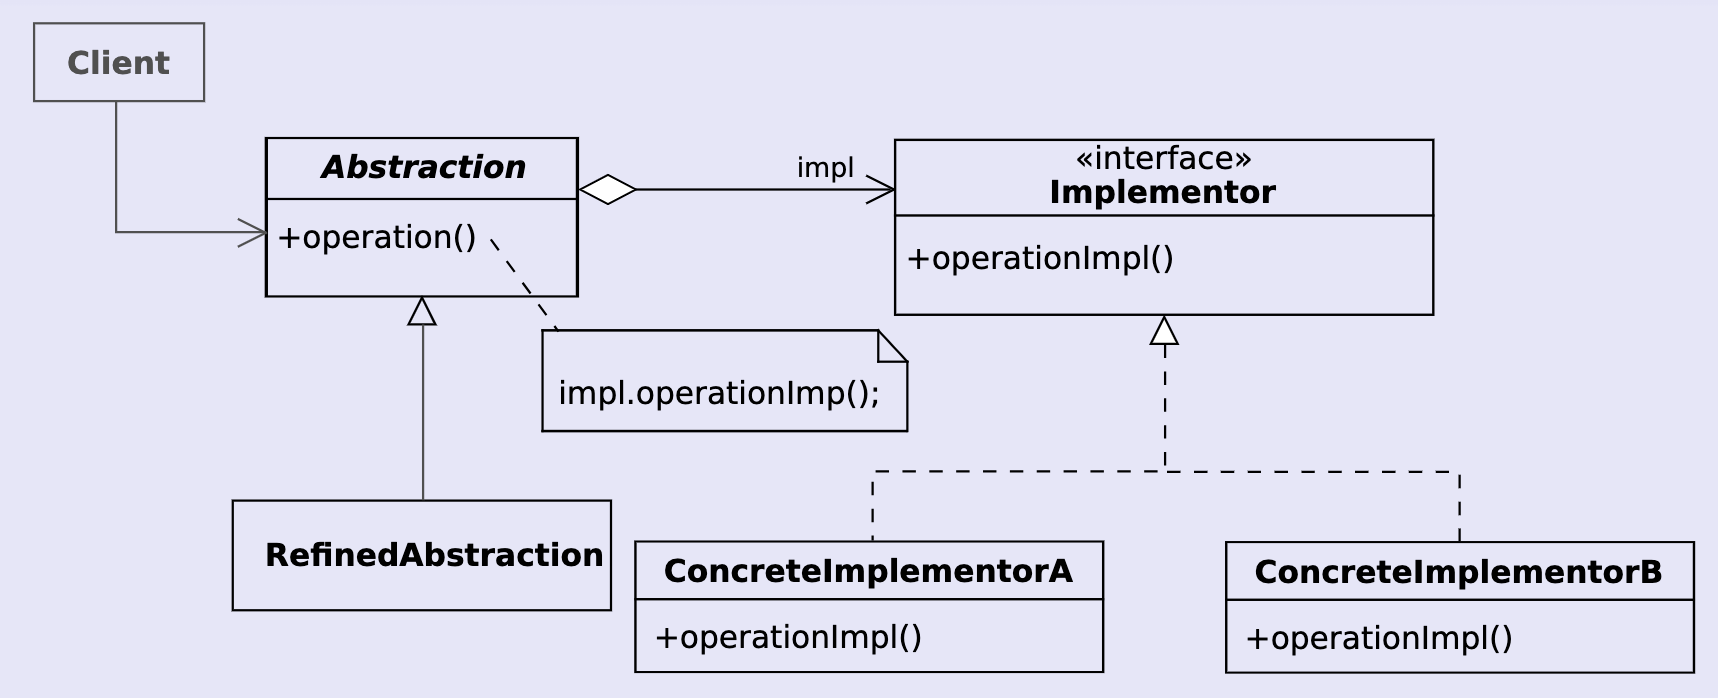
\includegraphics[width=1\linewidth]{assets/pattern/bridge/bridge-struttura.png}
\end{figure}

\paragraph{Struttura e Conseguenze} I partecipanti del pattern Bridge sono:
\begin{itemize}
    \item \textbf{Abstraction}: specifica l’interfaccia dell’astrazione. Mantiene un riferimento ad un oggetto di tipo Implementor;
    \item \textbf{RefinedAbstraction}: Estende l’interfaccia definita da Abstraction;
    \item \textbf{Implementor}: definisce l’interfaccia per le classi che implementano l’astrazione. Non deve corrispondere esattamente all’interfaccia di Abstraction: Implementor fornisce le operazioni base, mentre Abstraction definisce operazioni di più alto livello implementate sfruttando quelle di base;
    \item \textbf{ConcreteImplementor}: definisce un’implementazione concreta dell’interfaccia Implementor.
\end{itemize}

\begin{figure}[H]
    \centering
    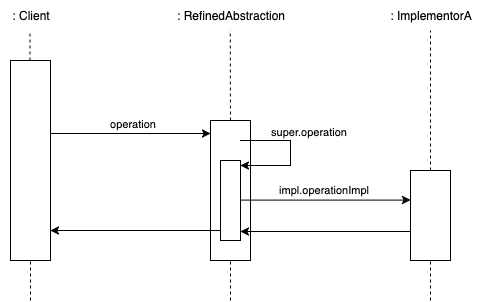
\includegraphics[width=1\linewidth]{assets/pattern/bridge/bridge-sequence.drawio.png}
    \caption{Sequence Diagram del pattern Bridge}
\end{figure}

L'utilizzo del pattern permette quindi maggiore \textbf{disaccoppiamento} tra interfaccia ed implementazione, maggiore \textbf{estensibilità} e mascheramento dei dettagli implementativi al client.

È possibile utilizzare Abstract Factory (\ref{abstract-factory}) per creare e configurare un particolare Bridge.

Il pattern Adapter (\ref{adapter}) permette di far cooperare classi non correlate a valle della loro implementazione.



\newpage